\documentclass[11pt,center]{beamer}

\usepackage{fancybox}
\usepackage{graphicx}
\usepackage{spot}
\usepackage{tikz}
\usepackage{minibox}
\usetikzlibrary{arrows}
\usepackage[absolute,overlay]{textpos}
\usetheme{metropolis}

\newcommand{\mli}[1]{\mathit{#1}}

\definecolor{light-gray}{gray}{0.86}
\title{\huge{Adaptive Machine Learning} \\ \large{Observing the regularities in the world}}
\author{Βασίλειος Αταλόγλου \\ Κωνσταντίνος Σαμαράς-Τσακίρης}
\date{\today}

\begin{document}

\begin{frame}%{\maketitle}
  \titlepage
\end{frame}

% Intro
\begin{frame}
  %Ο κόσμος παράγει δεδομένα. Τα αισθανόμαστε: ροές δεδομένων.
  %Τα δεδομένα αλλάζουν. Παράδειγμα ρομπότ;
  \centering
  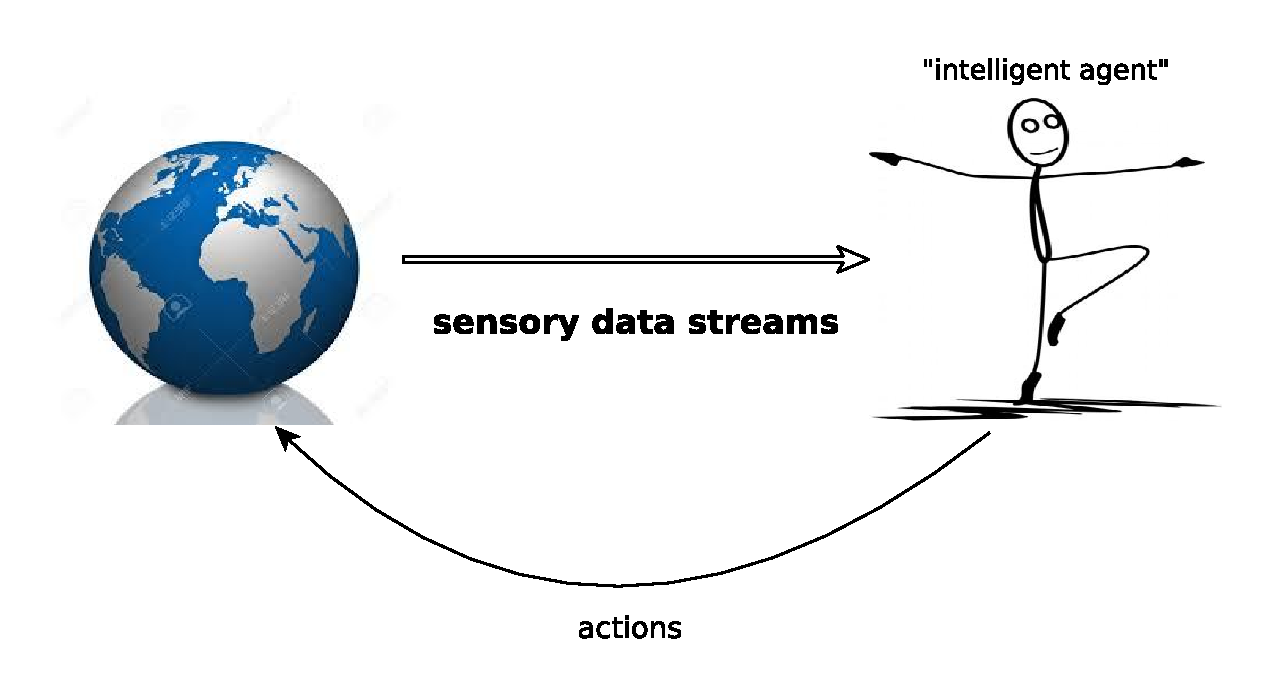
\includegraphics[width=0.8\textwidth]{../pics/world-man-interaction}
  \only<1-3>{\visible<2-3>{
	\begin{itemize}
	  \item Ζει μέσα στον κόσμο
	  \item Μαθαίνει τη δομή και τις βασικές αρχές του
	  \item ``Κοινή λογική''
	  \item<3>[] Και αυτά με τρόπο \em{unsupervised}, πραγματοποιώντας διαρκώς \em{προβλέψεις}.
	\end{itemize}
  }}
  \only<4->{ \includegraphics[width=0.65\textwidth]{../pics/angular_momentum} }
\end{frame}

\begin{frame}{Beyond the static \& supervised}
  %Στατική και supervised μάθηση δεν αρκεί. Πρόβλημα: αναγνώριση προτύπων σε ροές δεδομένων, sequence learning
  \begin{block}{Μοντελοποιώντας έναν κόσμο που αλλάζει}
	\pause
	\vspace{-0.5em}
	\begin{itemize}
	  \item Το μοντέλο πρέπει ή να είναι γενικό ή να προσαρμόζεται
	  \item Δεν είναι δυνατό να δημιουργηθούν labeled datasets -- υπερβολικός κόπος ή άγνοια
	  \pause
	  \item Τα δεδομένα έρχονται σε χρονική αλληλουχία (χρονοσειρές) \\ $\rightarrow$ Σχέσεις αιτιατότητας
	\end{itemize}
  \end{block}

  \pause
  \vspace{-0.5em}
  \begin{block}{Πρόβλημα: Sequence learning}
	Ο πράκτορας παρακολουθεί μια ακολουθία δεδομένων και καλείται να προβλέψει τη συνέχεια και να δράσει έτσι, ώστε να ανταμειφθεί. \\
	Κατ'επέκταση:
	\vspace{-0.3em}
	\begin{itemize}
	  \item Αναγνώριση ανωμαλίας
	  \item Λήψη αποφάσεων (κίνητρο παρέχεται από το περιβάλλον)
	\end{itemize}
  \end{block}
\end{frame}

\begin{frame}{How to do sequence learning}
  \begin{columns}
	\column{0.5\textwidth}
	\begin{itemize}
	  \item<2-> Hidden markov model
	  \item<3-> Time-delay neural network
	  \item<4-> Recurrent neural network
		\begin{itemize}
		  \item[--] LSTM
		\end{itemize}
	\end{itemize}
	\visible<5->{
	  \centering
	  \vspace{25pt}
	  \em\Large{Γενικότερο μοντέλο;}
	}
	\column{0.5\textwidth}
	\begin{itemize}
	  \item[]<2-> \includegraphics[width=0.8\textwidth]{../pics/hmm2}
	  \item[]<4-> \includegraphics[width=0.74\textwidth]{../pics/rnn}
	\end{itemize}
  \end{columns}
\end{frame}

\begin{frame}{Ανθρώπινος εγκέφαλος}
  O άνθρωπος έχει \alert{μνήμη} και μαθαίνει \alert{συνεχώς}, χωρίς επίβλεψη από το περιβάλλον.

  \pause
  \begin{columns}
	\column{0.7\textwidth}
	\\ Οι διαστάσεις του ανθρώπινου εγκεφάλου:
	\small{
	\begin{itemize}
	  \item[--] $10^{11}$ νευρώνες
	  \item[--] $10^4$ συνάψεις/νευρώνα
	  \item[--] $10$ σήματα/$sec$/σύναψη
	  \vspace{+0.5em}
	  \item Σύνολο: $10^{15}$ σήματα/$sec$
	  \item Ισχύς: $25$ Watt
	\end{itemize}
	}
	\column{0.3\textwidth}
	\\
	\includegraphics[width=1\textwidth]{../pics/brain.jpeg}
  \end{columns}

  \pause
  \begin{block}{}
	Οι δραστηριότητες που χαρακτηρίζουν τον άνθρωπο εντοπίζονται κυρίως στο \alert{neocortex}
  \end{block}
\end {frame}

\begin{frame}{Μοντελοποίηση μάθησης neocortex}
  Ανάγκη \alert{κατανόησης}
  \begin{itemize}
	\item Ο εγκέφαλος διαμορφώθηκε μέσω βιολογικής εξέλιξης και υπάγεται σε βιολογικούς περιορισμούς
	\item Ποιες είναι οι βασικές αρχές;
  \end{itemize}
  \visible<2->{
	Κάποιες παρατηρήσεις νευρολογίας neocortex:
	\begin{itemize}[]
	  \item<2-> Διδιάστατη μορφή χωρισμένη σε \alert{επίπεδα}
	  \item<3-> Δομή \alert{ομοιόμορφη} σε όλο το neocortex
		\begin{itemize} \item[--] Κάθε περιοχή λύνει το ίδιο πρόβλημα με τον ίδιο τρόπο \end{itemize}
	  \item<4-> Οι περιοχές ενώνονται \alert{ιεραρχικά}
		\begin{itemize} \item[--] Ψηλότερα επίπεδα => πιο αφηρημένες ιδέες \end{itemize}
	  \item<5-> Οι νευρώνες ενεργοποιούνται σποραδικά και πολύ σπάνια
		\begin{itemize} \item[--] Διάνυσμα κατάστασης: \spot<7>{\alert<5-6>{αραιό}} \end{itemize}
	  \item<6-> Συνεχής \alert{πρόβλεψη} του μέλλοντος με βάση τις αισθήσεις και τις μυϊκές εντολές
	\end{itemize}
  }
\end {frame}

\begin{frame}{Sparse Distributed Representation}
  \begin{block}{``Δομή δεδομένων του εγκεφάλου''}
	\begin{itemize}
	  \item Μεγάλο, αραιό διάνυσμα
	  \item Κάθε bit έχει \alert{νόημα}
	\end{itemize}
  \end{block}
\end{frame}

\begin{frame}{Ιδιότητες SDR}
    %\item Compressed storage
    %\item Similarity = intersection
    %\item Subsampling: 10 / 200
	%  \item Random match unlikely
	%  \item Partial match: generalization
	%\item Compare with union: set membership
  \begin{block}{Χωρητικότητα}
	Έστω το μέγεθος: $n$ και ο πληθυσμός των 1: $w$. Τα διαφορετικά SDRs με αυτή τη μορφή είναι $$ \binom nw= \frac{n!}{w!(n-w)!} $$
  \end{block}
  \pause
  \centering
  \large{Πώς μπορούμε να συνδυάσουμε/συγκρίνουμε 2 SDR?}
\end{frame}

\begin{frame}{Ταιριάζοντας SDRs}
  \only<1>{
  Έστω 2 SDR, το Α και το Β, ως boolean vectors:
  \begin{description}[Overlap set($w_b,b$)]
    \item[Union] $A | B$
    \item[Overlap] $A \& B$
    \item[Overlap score] Το μέτρο του overlap
    \item[Overlap set($w_b,b$)] Το σύνολο των SDR με πληθυσμό $w_b$ και overlap score $>b$ με το Α.
  \end{description}}
  \only<2->{
  \begin{description}[Matching($\theta$)]
    \item[Matching($\theta$)] Το Α και το Β ταιριάζουν, αν το overlap score τους είναι μεγαλύτερο από $\theta$
  \end{description}
  \begin{itemize}
	\item Έστω ότι Β = Α + 30\% θόρυβο. Τότε το εκτιμώμενο overlap score είναι $30\% \cdot w$. Αν $\theta = 30\% \cdot w$, τα Α και Β ταιριάζουν.
	\item \alert{Ευρωστία} στο θόρυβο!
	\item Πιθανότητα false positive: $8\times10^{-51}$ για $n=2048,\space w=41$
  \end{itemize}
  \pause
  $$p\{\mli{false\_positive}\}= \frac{|\mli{overlap\_set}|}{\mli{SDR\_capacity}}$$
  }
\end{frame}

\iffalse
\begin{frame} {Υποδειγματοληψία SDR}
  Συμπίεση: αποθηκεύονται μόνο θέσεις των 1

  \begin{block}{Υποδειγματοληψία}
	Έστω ότι αποθηκεύεται μόνο το 50\%.
	Αν συγκριθεί με τυχαίο SDR, η πιθανότητα false positive είναι πάρα πολύ μικρή.
  \end{block}
\end{frame}
\fi
\begin{frame} {Σύνολα από SDR}
  \begin{block}{Ερώτηση}
    Παρατηρούμε μια αλληλουχία από SDR. Πώς θα μάθουμε αν το ξεχωριστό SDR Β το έχουμε ξαναδεί;
  \end{block}

  \pause
  \vspace{1em}
  Εύκολο! \\
  Θα συγκίνουμε το Β με την \alert{ένωση} όλων των SDR

  \pause
  \vspace{0.5em}
  \centering
  \includegraphics[width=.5\textwidth]{../pics/balance}
\end{frame}


\begin{frame}{Neuron model}
  %Neuron with context
  %Minicolumn, layer: predictions, inhibitions
  \centering
  \includegraphics[width=.75\textwidth]{../pics/neuron-model}

  feedforward = receptive field
\end{frame}

\begin{frame}{Network model}
  \centering
  \includegraphics[width=\textwidth]{../pics/minicolumn}

  \vspace{-0.5em}
  \begin{block}{Συνδέσεις}
	Νευρώνες στο ίδιο minicolumn:
	\vspace{-0.5em}
    \begin{itemize}
      \item Tο ίδιο receptive field
      \item Μεταξύ τους inhibition
      \item[] $\rightarrow$ Winner-takes-all!
    \end{itemize}

	Μεταξύ διαφορετικών minicolumns:
	\vspace{-0.5em}
	\begin{itemize}
	  \item Context
	  \item Συνολικό inhibition
	\end{itemize}
  \end{block}
\end{frame}


\begin{frame}{Encoder}
\end{frame}

\begin{frame}{Spatial Pooler}
\end{frame}

\begin{frame}{Sequence memory}
  Example from paper
\end{frame}

\end{document}
